\section{Line-Of-Sight Propagation}\label{subsec:los_propagation}
\paragraph{}At low frequency (below approximately 3 MHz) radio signals travel as ground waves, which follow the Earth's curvature due to diffraction with the layers of the atmosphere.
However, neither of these effects are significant at higher frequencies and in lower levels of the atmosphere. Thus any obstruction between the transmitting antenna (transmitter) and the receiving antenna (receiver) will block the signal, just like the light that the eye may sense. Therefore, since the ability to visually see a transmitting antenna (disregarding the limitations of the eye's resolution) roughly corresponds to the ability to receive a radio signal from it, the propagation characteristic of VHF and higher radio frequency (>30 MHz) paths is called \textbf{Line-Of-Sight}. The farthest possible point of propagation is referred to as the \textbf{radio horizon}.

\paragraph{}The radio horizon is the locus of points at which direct rays from an antenna are tangential to the surface of the Earth. If the Earth were a perfect sphere and there were no atmosphere, the radio horizon would be a circle.
This way the greatest distance at which a receiver can see the transmitter is explained in the following paragraph.

\paragraph{}First, a general expression will be derived in order to, later on, apply it to a scenario with a UA and a GS. In Figure \ref{fig:GeometricDist_general} the relationship between the height of the observer above sea level (O point) and the distance, \textit{d}, is shown. Finding this distance is done by the use of the Pythagorean theorem. That is shown by the following equation:
\begin{equation}\label{eq:los_distToHorizon}
	(R+h)^2 = R^2+d^2\nonumber \\
	\Rightarrow R^2+2hR+h^2 = R^2+d^2 \Rightarrow d^2 = 2hR + h^2 \\
	\Rightarrow d = \sqrt{2hR + h^2}
\end{equation} 

\begin{figure}[H]
    \hfill
    \subfigure[Geometrical distance to the horizon.]{
    	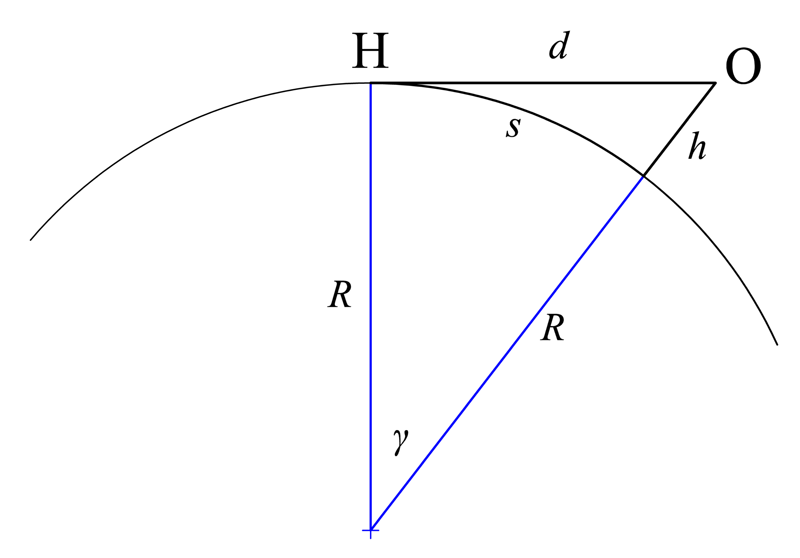
\includegraphics[scale=4]{figures/GeometricDistanceToHorizonOneTriangle.png} 
		\label{fig:GeometricDist_general}}
	\hfill
    \subfigure[Geometrical distance between UA and GS.]{
    	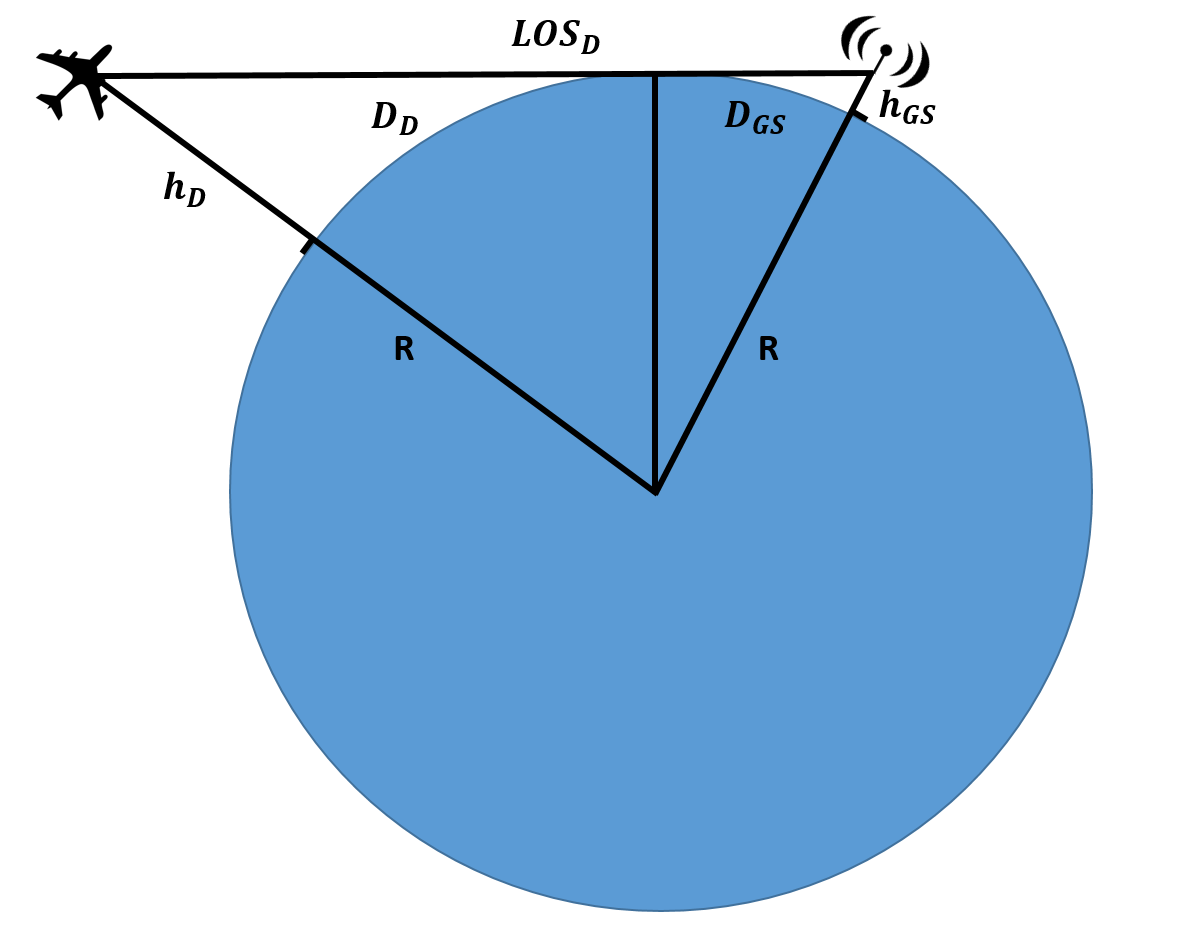
\includegraphics[scale=0.3]{figures/GeometricDistanceToHorizonTwoTriangle.png} 
    	\label{fig:GeometricDist_droneBasestation}}
    \hfill
    \caption{Line-Of-Sight calculations.}
\end{figure}

On Figure \ref{fig:GeometricDist_droneBasestation} it is shown that the two objects are a Ground Station and an drone. Both of them will not have an altitude bigger than approximately 100 meters and since \textit{R} is the radius of the Earth, $2hR$ >> $h^2$, and $h^2$ is therefore neglected in Equation \ref{eq:los_distToHorizon}. The two distances $D_D$ and $D_{GS}$ have the same expressions in both cases:
\begin{align*}
	D_D [km] &= \sqrt{2\cdot R \cdot h_D + h_{D}^2} \approx \sqrt{2\cdot 6.378\cdot h_D} = \sqrt{12.756\cdot h_D} = 3.57\cdot \sqrt{h_D[m]} \\
	D_{GS} [km] &= \sqrt{2\cdot R \cdot h_{GS} + h_{GS}^2} \approx \sqrt{2\cdot 6.378\cdot h_{GS}} = \sqrt{12.756\cdot h_B} = 3.57\cdot \sqrt{h_{GS}[m]}
\end{align*}

Now, with these derivations, the maximum distance at which both Ground Station and UA are still able to see each other ($LOS_{d}$), and therefore keep the communication, can be calculated as:
\begin{align}
	LOS_d[km]	 &= D_D + D_{GS} \approx 3.57\cdot \sqrt{h_D[m]} + 3.57\cdot \sqrt{h_{GS}[m]} = {3.57\cdot (\sqrt{h_D[m]} + \sqrt{h_{GS}[m]}} )
\end{align}

\subsection*{LOS Distance Example}
A simple but realistic example scenario would be where the aircraft is at $h_D = 100$m and the ground station at $h_B = 20$m. This maximum distance between them is as follows:
\begin{equation*}
	LOS_d = 3.57\cdot (\sqrt{100} + \sqrt{20}) = 51.67 \text{ km}
\end{equation*}

During the course of this document this number might sometimes appear as an upper limit for the maximum distance since, further than that, there would not be Line-Of-Sight connection. Increasing this distance would be resulting from either increasing the altitude of the drone or of the Ground Station. However, both of these approaches not viable. The altitude of the drone is restricted by the Danish Aviation Law and increasing the altitude of the GS would involve setting it up in a very high building or mountain.




